% ==============================
% 一、实验目的
% ==============================

\section{实验目的}

\begin{enumerate}[label=\arabic*、, leftmargin=4em, labelsep=0pt]
    \item 学习金相试样的制备方法，了解金相显微组织的显示方法；
    \item 了解金相显微镜的基本光学原理和主要构造；
    \item 掌握金相显微镜的正确使用方法；
    \item 利用金相显微镜观察铁碳合金（球墨铸铁、20钢、纯铁）的显微组织，并进行分析。
\end{enumerate}

% ==============================
% 二、显微镜的基本原理和主要结构
% ==============================

\section{显微镜的基本原理和主要结构}

\subsection{基本光学放大原理}

金相显微镜利用两平行凸透镜组成透镜组进行放大。如图2-1所示，物体AB经物镜和目镜两级放大后，在人眼中形成颠倒放大的物象A''B''。显微镜的总放大倍数$M$为物镜放大倍数与目镜放大倍数的乘积：

\begin{equation}
    M = M_{\text{物镜}} \times M_{\text{目镜}}
\end{equation}

物镜最高放大倍数可达100倍，目镜放大倍数可达25倍。例如，物镜$40\times$配合目镜$10\times$，则总放大倍数为$400\times$。

\begin{figure}[H]
    \centering
    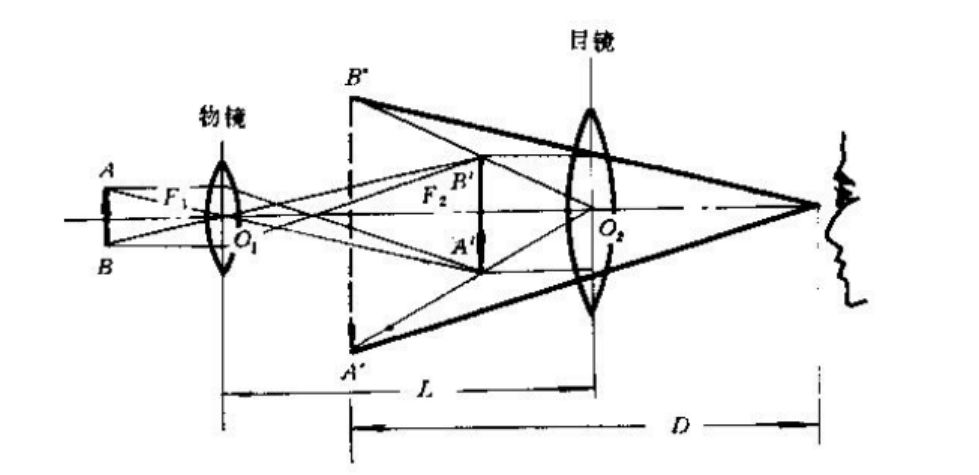
\includegraphics[width=0.7\textwidth]{data/放大原理图.png}
    \caption{显微镜的光学放大原理示意图}
    \label{fig:optical-principle}
\end{figure}

\subsection{显微镜的基本构造}

显微镜种类繁多，常见的有台式、立式和卧式三种，基本由光学系统、照明系统和机械系统三大部分组成。

\begin{figure}[H]
    \centering
    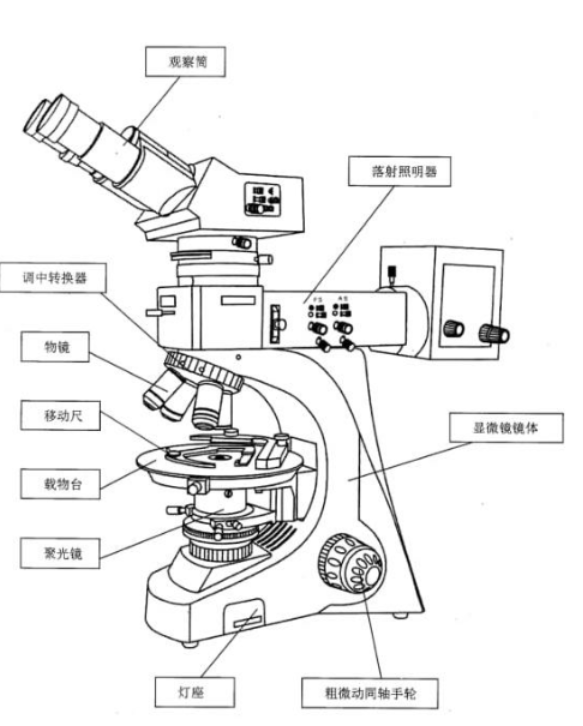
\includegraphics[width=0.6\textwidth]{data/结构示意图.png}
    \caption{59XF偏光显微镜结构示意图}
    \label{fig:microscope-structure}
\end{figure}

\textbf{主要技术参数：}

\begin{itemize}[leftmargin=2em]
    \item 光学系统：无限远消应力平场校正系统；
    \item 目镜：高眼点大视野平场目镜 PL10X/22mm；
    \item 物镜：无限远长工作距消应力平场物镜（5X/10X/20X/50X），10X目镜下实现50X--500X放大；
    \item 载物台：直径160mm，可360°旋转，格值1°；
    \item 调焦机构：粗微同轴调焦，粗调行程30mm，微调精度0.002mm；
    \item 光源：自适应宽电压100--240V，12V 50W柯拉照明。
\end{itemize}

% ==============================
% 三、显微镜的使用方法及注意事项
% ==============================

\section{显微镜的使用方法及注意事项}

\subsection{使用方法}

\begin{enumerate}[label=（\arabic*）, leftmargin=4em, labelsep=0pt]
    \item 将显微镜光源通过低压变压器接通电源；
    \item 根据所需放大倍数选择并安装物镜和目镜，使转换器旋转至固定位置；
    \item 将试样放在载物台中心，观察面朝上；
    \item 选择反射照明模式，转动粗调手轮使镜筒上升，使物镜接近试样表面，再反向转动手轮使镜筒逐渐下降；当视场亮度增强时改用细调手轮，直至物象清晰为止；
    \item 适当调节孔径光栏和视场光栏，以获得最佳图像质量；
    \item 用手轻轻推动载物台，选择所需观察的视场。
\end{enumerate}

\subsection{注意事项}

\begin{enumerate}[label=（\arabic*）, leftmargin=4em, labelsep=0pt]
    \item 小心操作，光学系统不能自行拆卸；
    \item 镜头玻璃部分和试样表面不能用手直接接触，灰尘可用镜头纸轻轻擦净；
    \item 旋转调焦手轮时动作要慢，碰到阻碍时不得强行转动；
    \item 使用完毕后应及时关闭电源，盖上防尘罩。
\end{enumerate}

% ==============================
% 四、金相试样的制备过程
% ==============================

\section{金相试样的制备过程}

\subsection{实验材料与设备}

\begin{itemize}[leftmargin=2em]
    \item \textbf{金相试样}：球墨铸铁、20钢、纯铁；
    \item \textbf{金相砂纸}：320\#、400\#、600\#、800\#、1000\#、1200\#、1500\#；
    \item \textbf{腐蚀剂}：3--4\%硝酸酒精溶液；
    \item \textbf{其他}：玻璃板、玻璃皿、棉签、酒精、脱脂棉、吹风机（冷风档）。
\end{itemize}

\subsection{制备步骤}

金相试样的制备主要包括粗磨、中磨、细磨和腐蚀四个阶段。

\textbf{1. 清洁与准备}

清洁试样表面油污，检查砂纸平整无破损，按粗到细顺序摆放，确保磨制平台干净平整。

\textbf{2. 粗磨（去除切割损伤层）}

将砂纸平铺于稳固平台，手持试样均匀施压，沿单一方向推磨（切勿来回摩擦）。每磨数下将试样旋转90°，以改变磨痕方向并确保磨面均匀。磨至表面布满均匀、方向一致的划痕后，吹净磨屑，避免粗颗粒带入下一道工序。

\textbf{3. 中磨（消除粗划痕）}

换用更细砂纸，将试样旋转90°后沿单一方向均匀磨制，直至上一道粗划痕完全消失，被更细、更均匀的划痕取代。在良好光线下侧视，应仅看到当前砂纸的划痕。

\textbf{4. 细磨（获得精细划痕）}

逐级更换砂纸（600\#→800\#→1000\#→1200\#→1500\#），每次更换前将试样旋转90°，施压逐渐减轻。最终磨痕应均匀细密、方向一致，上一道砂纸的划痕完全消失，表面平整无浮雕、塌边。

\textbf{5. 腐蚀}

将磨好的试样浸入硝酸酒精溶液中。腐蚀时间因材料而异：

\begin{itemize}[leftmargin=2em]
    \item \textbf{球墨铸铁}：3--10秒，显示石墨球和基体组织；
    \item \textbf{20钢}：10--30秒，显示铁素体和珠光体；
    \item \textbf{纯铁}：30秒--2分钟，显示铁素体晶界。
\end{itemize}

\noindent\textbf{关键原则：宁浅勿深。}腐蚀后立即用水冲洗，酒精棉球擦拭并吹干，即可进行显微镜观察。

% ==============================
% 五、显微组织观察结果
% ==============================

\section{显微组织观察结果}

\subsection{纯铁}

纯铁含碳量在0.02\%以下，组织为等轴多边形铁素体晶粒，晶界平直。经浅腐蚀后晶界呈细黑线显现。

\begin{figure}[H]
    \centering
    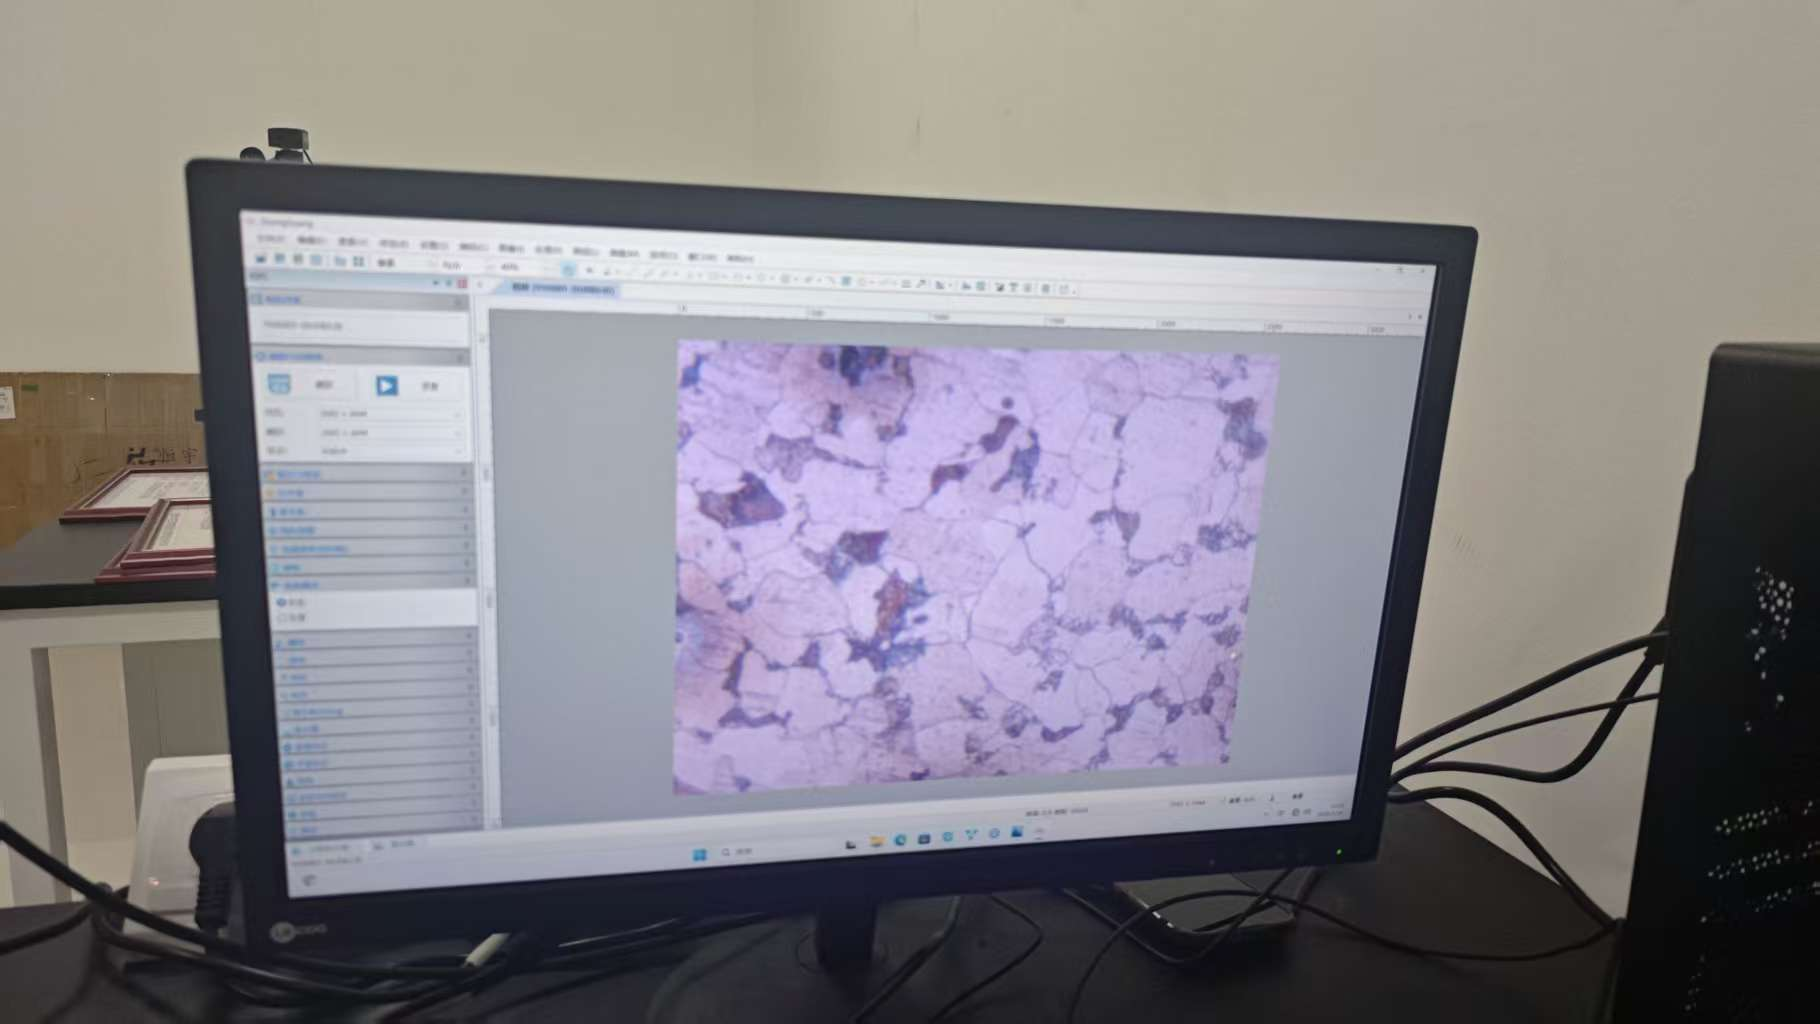
\includegraphics[width=0.7\textwidth]{data/纯铁式样.jpg}
    \caption{纯铁显微组织}
    \label{fig:pure-iron-photo}
\end{figure}